% Results sections of the supplement. Every number is a macro or table generated by scripts/make_tables.py from results/*.json.
% Every result is a MODEL PREDICTION conditional on the literature anchors of Sec. 3, not a measurement.

\section{Predicted performance of published and own designs}\label{sec:pred}
All numbers of this section are means over the \nDesignWorlds{} literature-consistent worlds (24 devices $\times$ 3 oxidation-depth nodes each); ``yield'' is the hard yield of Sec.~\ref{sec:model}.
The designs are those of the published experiments \cite{yuan2025apl126,yuan2025clea} and the 16 designs of the author's mask (families A and B, eight rotations; Sec.~\ref{sec:falsify}).
\begin{table}[H]\centering\small\tabDesigns
\caption{Predicted yield per design. The bracket gives the 10th and 90th percentile over worlds: the spread between worlds is as large as the differences between designs, so a ranking is a statement about probabilities, not about one wafer.}\label{tab:designs}\end{table}
\begin{figure}[H]\centering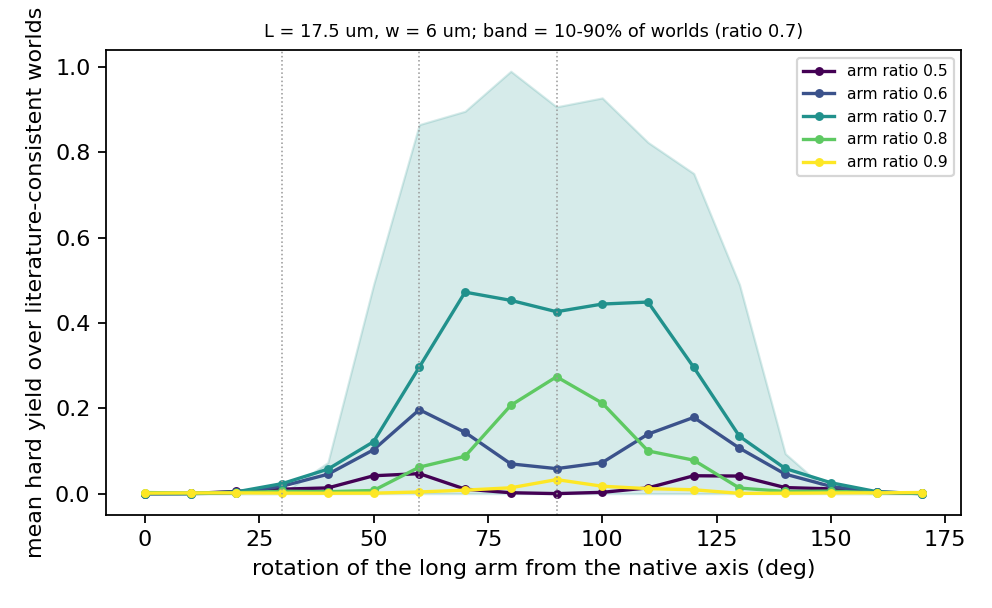
\includegraphics[width=0.62\textwidth]{figures/rotation_scan.png}\caption{Rotation scan for five arm ratios ($L=17.5\,\mu$m, $w=6\,\mu$m, $\rho=0.5$): mean hard yield over the literature-consistent worlds; the band is the 10--90\,\% range for arm ratio 0.7.}\label{fig:rot}\end{figure}
\begin{figure}[H]\centering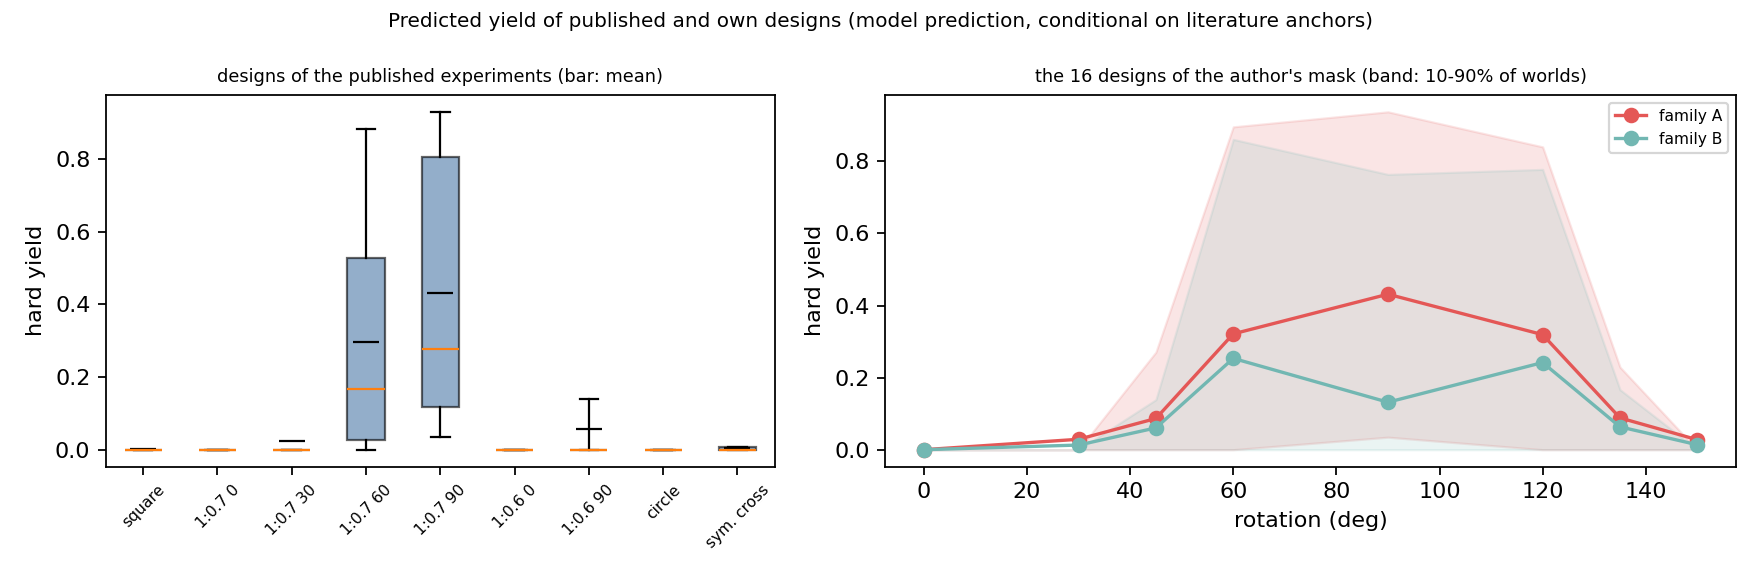
\includegraphics[width=\textwidth]{figures/designs.png}\caption{Yield of the designs of the published experiments (left) and of the 16 designs of the author's mask (right).}\label{fig:designs}\end{figure}

\paragraph{Arm ratio and rotation.} For the 1:0.7 cross the mean yield is at least 90\,\% of its maximum (\meanYieldSevenMax) for rotations between \plateauLo$^\circ$ and \plateauHi$^\circ$ (Fig.~\ref{fig:rot}); it is near zero at $0^\circ$ (long arm along the native axis, no compensation), small at $30^\circ$ and still on a steep flank at $60^\circ$.
The share of worlds in which some rotation of the cross (at $L=17.5$, $w=6$) reaches a yield of 0.5 depends strongly on the arm ratio: \reachRatioFive\,\% (0.5), \reachRatioSix\,\% (0.6), \reachRatioSeven\,\% (0.7), \reachRatioEight\,\% (0.8), \reachRatioNine\,\% (0.9).
Part of this peak at 0.7 is built into the anchors, which were formulated with the 1:0.7 and 1:0.6 designs of the experiments; it is a property of the \emph{conditional} model, not an independent confirmation that 0.7 is optimal.
\begin{table}[H]\centering\small\tabTopSeven
\caption{Among the seven designs of \cite{yuan2025apl126}: the share of worlds in which each is the best one (ties broken toward the smaller index). In \noWorkingSeven\,\% of the worlds none of the seven is a working device.}\label{tab:top7}\end{table}
\paragraph{Does the ranking of rotations depend on what counts as a good switching current?} Yes, and this matters for the answer below. The yield requires one switch inside a window of $\mu=I/I_{th}$, which is a specification of the node, not a physical constant.
Table~\ref{tab:window} scores the 1:0.7 cross at rotations from $40^\circ$ to $90^\circ$ in \nWindowWorlds{} worlds (every second literature-consistent world) under four windows.
\begin{table}[H]\centering\small\tabWindow
\caption{Mean yield of the 1:0.7 cross ($L=17.5$, $w=6\,\mu$m, $\rho=0.5$) at rotations from the native axis, for four switching-current windows (default 1.25--1.95; low bias 1.15--1.60; wide 1.15--2.05; narrow 1.50--1.70), and the share of worlds in which the $60^\circ$ device beats the $90^\circ$ one and vice versa (ties excluded).}\label{tab:window}\end{table}

\paragraph{Which aperture is best for polarization switching in an Ising node? What the evidence supports.}
\emph{Experiments} \cite{yuan2025apl126}: the text I read reports injection-locking power for the 1:0.7 cruciform rotated by $60^\circ$ (248\,$\mu$W at 10\,mA; 3.6\,$\mu$W just above threshold) and for the non-switchable square (371\,$\mu$W at 10\,mA); it does not rank all seven designs. The $30^\circ$, $60^\circ$ and $90^\circ$ cruciforms are grouped as switching devices.
That is a measurement of injection-locking power on the devices shown, not a yield, and the number of devices per design is not stated in the text I could read.
\emph{This model}, conditional on the anchors: among the designs of the published experiments only the 1:0.7 crosses at $60^\circ$ and $90^\circ$ have a substantial yield (Table~\ref{tab:designs}); the yield of a 1:0.7 cross rises steeply between $50^\circ$ and $70^\circ$, has a broad plateau between $70^\circ$ and $110^\circ$ (the mirror image of $70^\circ$--$80^\circ$ is $100^\circ$--$110^\circ$), inside which there is no reliable ranking of the rotations, and falls again beyond it. The best rotation is $70^\circ$ or $80^\circ$ in all four windows (Table~\ref{tab:window}); across the alternative ways of conditioning on the literature of Sec.~\ref{sec:sens} (Table~\ref{tab:rotsets}) the plateau is the same but its maximum moves, and $80^\circ$ (equivalently $100^\circ$) is the safest single rotation, though narrowly (Sec.~\ref{sec:sens}).
The $90^\circ$ device is close to the best rotation for the default, wide and narrow windows, but it loses about 40\,\% of its yield when switching at low bias is required, where the $60^\circ$ device is as good or better ($60^\circ$ beats $90^\circ$ in \lowBiasSixtyBeatsNinety\,\% of the worlds against \lowBiasNinetyBeatsSixty\,\% for the reverse; for the default window \defSixtyBeatsNinety\,\% against \defNinetyBeatsSixty\,\%).
This is not in conflict with the injection-locking measurement of the $60^\circ$ device, which was made just above threshold as well as at 10\,mA, but it means that ``the $60^\circ$ device was best'' and ``the $70^\circ$--$80^\circ$ device is the most robust choice'' are answers to different questions; \textbf{the mask of Sec.~\ref{sec:falsify} contains $60^\circ$, $90^\circ$ and $120^\circ$ and can inform it, but not $70^\circ$--$80^\circ$}. Restricted to the interior of the search box, the first two additions that the model would make to the mask are crosses at $70^\circ$ and $80^\circ$ (Table~\ref{tab:addint}); the first unrestricted addition is a thin-armed design at $85^\circ$ on the wall of the box.
\emph{Beyond the published designs}, the batch search of Sec.~\ref{sec:batch} favours thin-armed crosses with a small arm ratio near $85^\circ$--$90^\circ$; they lie at the edge of the search box, where the reduced model is least reliable (Sec.~\ref{sec:batch}), and are hypotheses, not recommendations.
A ranking that is meaningful for the wafer at hand requires measured constants (Sec.~\ref{sec:falsify}).

\section{Optimiser benchmark}\label{sec:bench}
\textbf{Question.} Does Bayesian optimisation find better apertures than random search, Sobol points and differential evolution for the same number of simulations (48)?
\textbf{Problems.} \emph{P1}: the wafer constants are known (one of five literature-consistent worlds), default window for the switching current ($\mu_{sw}\in[1.25,1.95]$). The five wafers were chosen among 30 accepted worlds: those in which no design of a 128-point Sobol cloud reaches a yield of 0.6 were dropped and five spanning the range of difficulty were kept, so they are not a random sample of the accepted worlds.
\emph{P2}: as P1 with a narrow window $[1.50,1.70]$ (good designs are rarer). \emph{P3}: the constants are unknown; one design is chosen to maximise the mean smoothed yield over 8 literature-consistent worlds and is scored on 24 \emph{unseen} worlds --- the situation before the first batch is measured.
\textbf{Methods.} Random search, scrambled Sobol points, differential evolution \cite{storn1997}, and Bayesian optimisation with a Gaussian-process surrogate \cite{rasmussen2006} (Mat\'ern-5/2 kernel with one length scale per input, white noise; scikit-learn \cite{pedregosa2011}; the rotation enters as $(\cos2\theta,\sin2\theta)$ so that the $180^\circ$ periodicity is exact),
with Expected Improvement \cite{jones1998} or the upper confidence bound \cite{srinivas2010,snoek2012} maximised over the design box.
\textbf{Protocol.} The optimisers see the smoothed yield on one fixed device population (common random numbers). The reported quality is the hard yield of the returned design on a \emph{fresh} population of 96 devices (and, for P3, on unseen worlds), so no method benefits from optimism about the sample it saw.
Paired Wilcoxon tests and bootstrap intervals are computed over (world, seed) pairs; \nRunsPone{} runs per method for P1 and \nRunsPthree{} for P3, 40 for P2.
\begin{table}[H]\centering\small\tabBench\caption{Mean held-out hard yield [95\,\% bootstrap interval] of the design returned by each method.}\label{tab:bench}\end{table}
\begin{table}[H]\centering\small\tabTests\caption{Paired differences (method minus baseline) of the held-out yield.}\label{tab:tests}\end{table}
\begin{figure}[H]\centering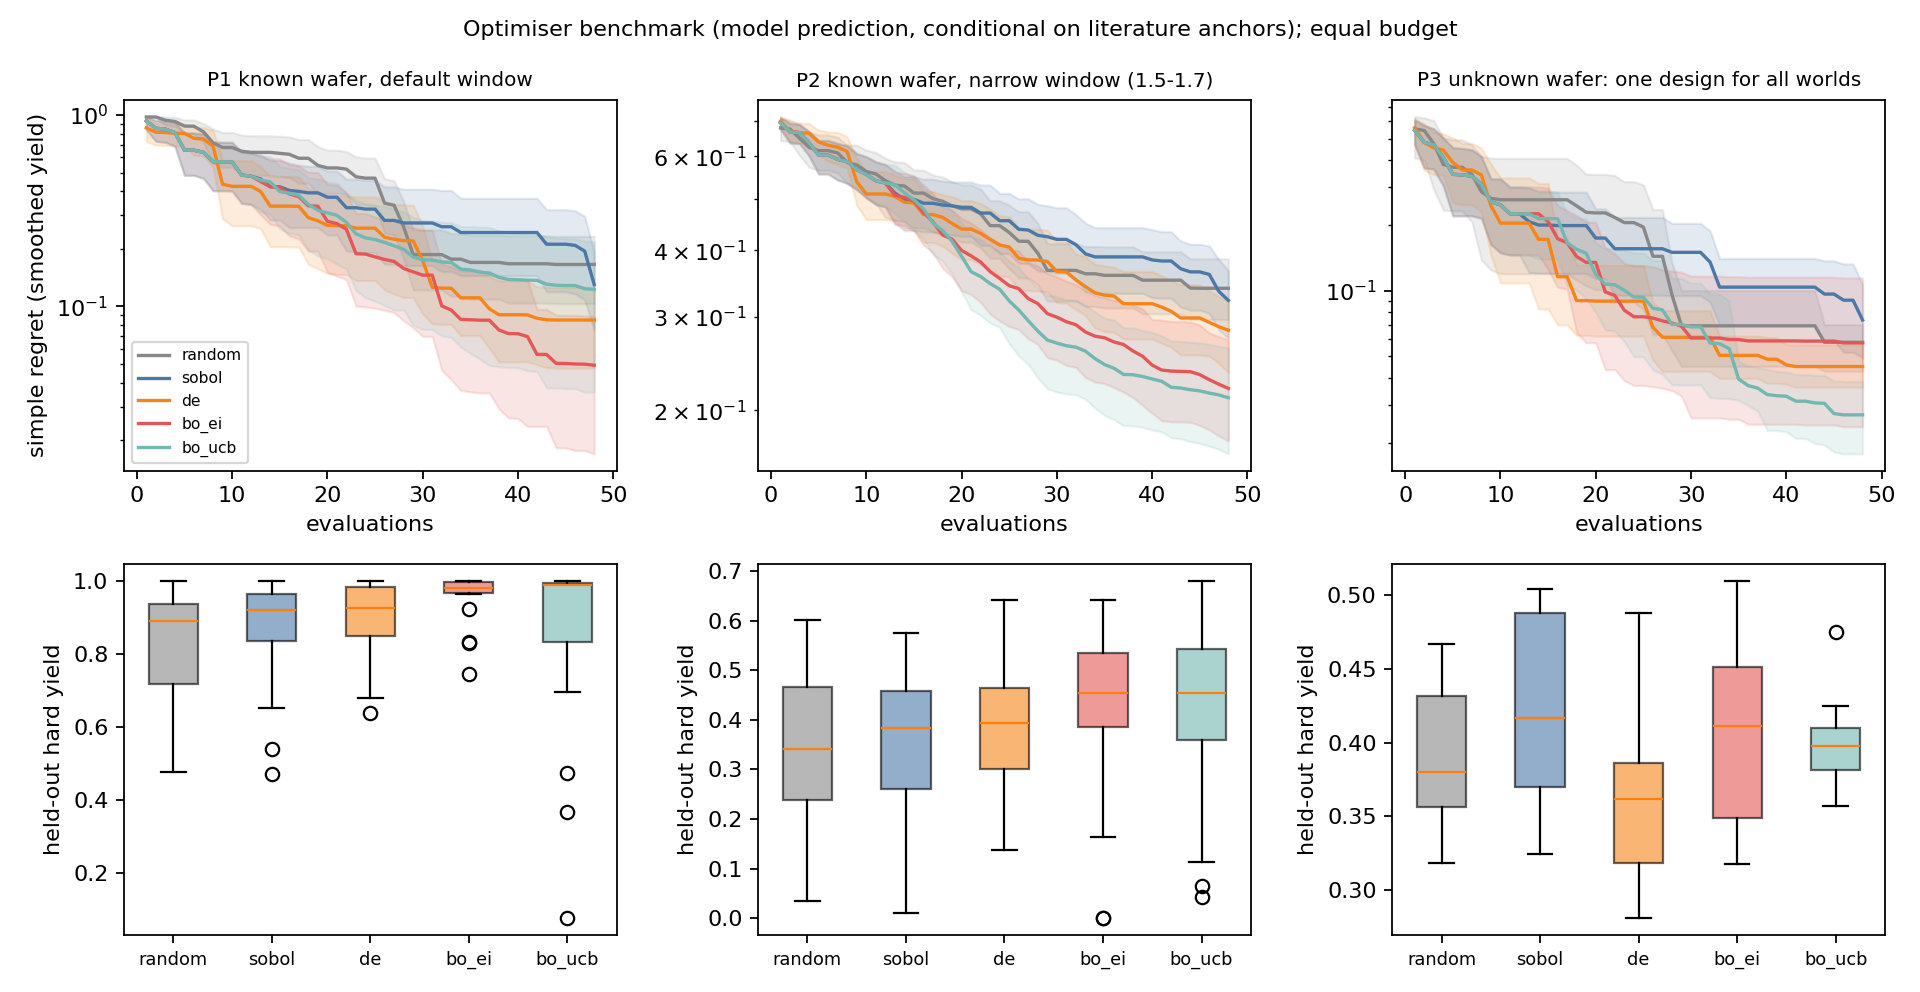
\includegraphics[width=\textwidth]{figures/benchmark.png}\caption{Top: simple regret of the smoothed yield against the best value found by any run in the same world (mean and bootstrap band). Bottom: held-out hard yield.}\label{fig:bench}\end{figure}
\paragraph{Reading of Tables~\ref{tab:bench} and~\ref{tab:tests}.}
\emph{P1 (wafer known, default window).} GP-EI returns designs with a held-out yield of \benchOneBoEi{}, against \benchOneRandom{} for random search, \benchOneSobol{} for Sobol points and \benchOneDe{} for differential evolution; all three differences are significant in paired Wilcoxon tests (\diffOneBoEiRandom{}, $p=\pvalOneBoEiRandom$; \diffOneBoEiSobol{}, $p=\pvalOneBoEiSobol$; \diffOneBoEiDe{}, $p=\pvalOneBoEiDe$; \nRunsOne{} paired runs, not corrected for six comparisons, and runs within one world are not independent).
At the level of the five wafers (the four seeds of a wafer averaged; Table~\ref{tab:wafer}) GP-EI is ahead of random search and of Sobol points on all five wafers (mean difference over wafers \waferOneBoEiRandom{} and \waferOneBoEiSobol{}, 95\,\% $t$-interval) and of differential evolution on \waferAheadOneBoEiDe{} of 5 (\waferOneBoEiDe{}); with only five wafers the interval excludes zero for random search but includes it for Sobol points (marginally) and for differential evolution.
GP-UCB is less reliable: its mean (\benchOneBoUcb{}) is not significantly above random search ($p=\pvalOneBoUcbRandom$), because \lowRunsOneBoUcb{} of its \nRunsOnePerMethod{} runs return a design with a yield below 0.5 (GP-EI: \lowRunsOneBoEi{}; random search: \lowRunsOneRandom{}).
In those runs the best value that the optimiser itself had seen on its own device population was also low (\ucbLowBestMin--\ucbLowBestMax), so they had not converged within 48 evaluations (the fixed exploration weight $\beta=2$ is the likely reason; I did not test other weights) rather than over-fitted the population.
\emph{P2 (wafer known, narrow window).} Both Bayesian optimisers return designs with a held-out yield of \benchTwoBoEi{} (GP-EI) and \benchTwoBoUcb{} (GP-UCB), against \benchTwoRandom{} for random search, \benchTwoSobol{} for Sobol points and \benchTwoDe{} for differential evolution.
The gain over random search (\diffTwoBoEiRandom{}, $p=\pvalTwoBoEiRandom$) and over Sobol points (\diffTwoBoEiSobol{}, $p=\pvalTwoBoEiSobol$) is significant in paired Wilcoxon tests (not corrected for six comparisons; the GP-UCB values are in Table~\ref{tab:tests});
the gain over differential evolution (\diffTwoBoEiDe{}, $p=\pvalTwoBoEiDe$ for GP-EI; \diffTwoBoUcbDe{}, $p=\pvalTwoBoUcbDe$ for GP-UCB) is not.
By world, the better Bayesian optimiser leads differential evolution by more than 0.02 in \worldsBoAheadDeTwo{} of the \nWorldsTwo{} worlds, is level in \worldsTieBoDeTwo{} and trails in \worldsDeAheadBoTwo{}; the eight seeds of one world are not independent draws of the problem, so the tests overstate the effective sample size.
At the level of wafers (Table~\ref{tab:wafer}) GP-EI is ahead of random search on \waferAheadTwoBoEiRandom{} and of Sobol points on \waferAheadTwoBoEiSobol{} of 5 wafers, GP-UCB on \waferAheadTwoBoUcbRandom{} and \waferAheadTwoBoUcbSobol{}; the interval over wafers excludes zero for GP-EI against random search and for GP-UCB against random search and Sobol points, and includes it in every comparison with differential evolution.
\begin{table}[H]\centering\small\tabWafer\caption{Optimiser benchmark at the level of wafers: the seeds of a wafer are averaged and the five wafer means are compared (mean difference of the held-out yield, 95\,\% $t$-interval over wafers, number of wafers in which the Bayesian optimiser is ahead).}\label{tab:wafer}\end{table}
\emph{P3 (wafer unknown; one design for eight worlds, scored on 24 unseen worlds).} The five methods lie between \benchThreeMin{} and \benchThreeMax{} and no difference is significant (Friedman test over the five methods, $p=\friedThree$; \nRunsThree{} runs per method, so differences of a few hundredths could not be detected).
All five methods lose about the same amount between the eight selection worlds (\pThreeSelLo--\pThreeSelHi, the yield of the returned design on those worlds) and the 24 unseen ones (\pThreeUnseenLo--\pThreeUnseenHi; a loss of \pThreeGapLo--\pThreeGapHi): a design tuned on eight worlds mostly over-fits them, whichever search algorithm produced it, and with eight runs per method the test has little power.
This is the situation that motivates the batch of Sec.~\ref{sec:batch}, whose score is a different quantity: the expected best-of-batch yield (0.86 on 32 unseen worlds, \othPortOther{} on \nOtherWorlds{} further ones) assumes that the best design of the batch can be identified after measurement and is not comparable with the yield of one design.
P3 does not show that a single design cannot hedge: the best single design of the pool, chosen on 32 training worlds, reaches \singleBestYield{} on 32 other worlds (Table~\ref{tab:batch}), although it lies on a wall of the search box.
\emph{What this does not show.} A simulator evaluation costs a fraction of a second, so the budget of 48 is a statement about sample efficiency, not about cost; a fabrication run is many orders of magnitude more expensive and the real batch is 16 designs.
The optimiser and the scoring use the same reduced model, so the benchmark says nothing about how well the model represents devices.

\section{Designing a fabrication batch}\label{sec:batch}
A mask is a batch: the 16 designs are fixed before any measurement, and the constants of the wafer are still unknown. The batch is therefore chosen to maximise the \emph{expected best yield in the batch},
$E_w[\max_j Y_j(w)]$ over worlds $w$, a monotone submodular set function that a greedy algorithm maximises within a factor $1-1/e$ of the optimum \cite{nemhauser1978}.
\textbf{Candidates:} \nPool{} designs (128 Sobol points; the best designs of two prior-robust Bayesian-optimisation runs; the nine reference designs; the author's 16; a rotation family). \textbf{Selection:} on \nTrainWorlds{} \emph{training} worlds only.
\textbf{Scoring:} on \nTestWorlds{} disjoint \emph{test} worlds (all worlds are literature-consistent, so the test worlds share the assumptions of the training worlds; they are unseen constants, not an independent check of the model).
This is not the batch Bayesian optimisation of \cite{desautels2014}, which spreads a batch over a Gaussian-process posterior; that alternative was not compared.
\begin{table}[H]\centering\small\tabBatch\caption{Expected best-of-batch yield on unseen worlds. In \noWorkingTest{} of the \nTestWorlds{} test worlds no design of the pool reaches a yield of 0.3.}\label{tab:batch}\end{table}
\begin{table}[H]\centering\small\tabMaskPlus\caption{Adding $k$ designs (chosen on the training worlds) to the author's 16-design mask.}\label{tab:maskplus}\end{table}
\begin{table}[H]\centering\small\tabAdd\caption{The added designs of Table~\ref{tab:maskplus}, in the order of the greedy choice.}\label{tab:add}\end{table}
\begin{table}[H]\centering\small\tabBatchList\caption{The 16 designs of the portfolio (lengths in $\mu$m, $\rho$ = corner rounding, $\theta$ = rotation in degrees), with their yield on training and test worlds.}\label{tab:batchlist}\end{table}
\begin{figure}[H]\centering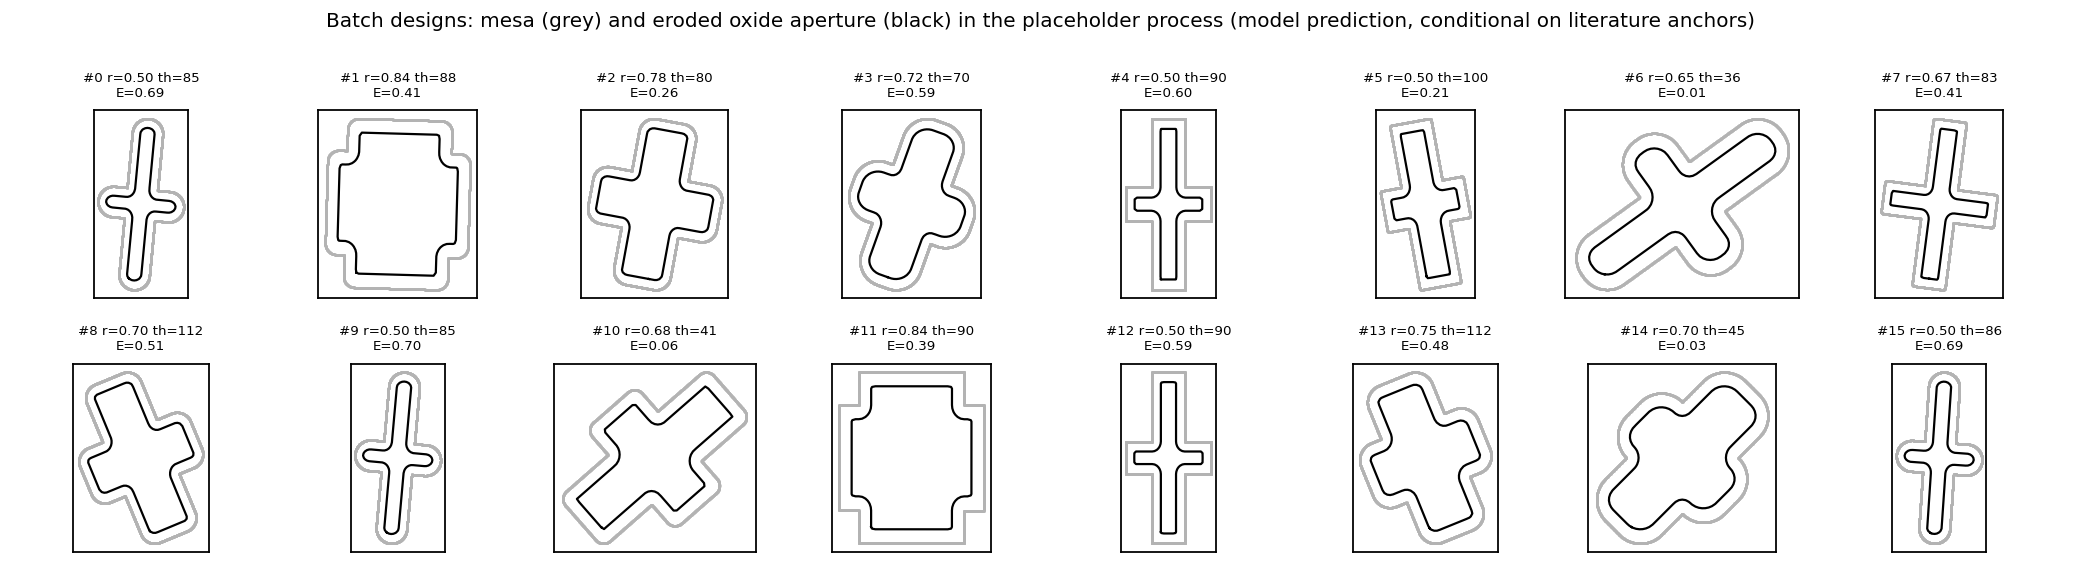
\includegraphics[width=\textwidth]{figures/batch_shapes.png}\caption{The portfolio: mesa (grey) and eroded oxide aperture (black) in the placeholder process.}\label{fig:batch}\end{figure}
\paragraph{Boundary and fresh-device checks.} \nWall{} of the \nQ{} portfolio designs sit on a wall of the search box (thinnest arms and/or lowest arm ratio); their oxide apertures have an area of only \wallAreaLo--\wallAreaHi\,$\mu$m$^2$
against \refAreaLo--\refAreaHi\,$\mu$m$^2$ for the cruciforms of the experiments and \circleArea\,$\mu$m$^2$ for the circle (Table~\ref{tab:walls}). Thin arms are where the scalar-mode, single-mode description is least credible and where loss and current density that the model does not contain would matter.
Two checks were made on the same test worlds: (i) the sets were re-scored on a new population of \freshDev{} devices, so that the comparison cannot come from over-fitting to particular device draws; (ii) a portfolio was re-selected from the \nPoolInterior{} candidates of the pool inside a conservative interior box (arm ratio $\ge0.6$, $4.5\le w\le7.5\,\mu$m, $13\le L\le19\,\mu$m).
\begin{table}[H]\centering\small\tabInterior\caption{Fresh device population; same unseen worlds.}\label{tab:interior}\end{table}
\begin{table}[H]\centering\small\tabWalls\caption{Portfolio designs with the area of their oxide aperture in the placeholder process.}\label{tab:walls}\end{table}
The advantage of the model-selected batch over the author's mask and over the seven published designs survives both checks (Table~\ref{tab:interior}); the interior-only batch gives up part of it (\interiorSame{} on the original devices), which is the price of staying where the model is credible.
\paragraph{What the batch tells the author about her mask.} Most of the value comes from a few designs: the first four designs of the greedy order already reach 0.81 on the training worlds and the first eight give nearly the same expected best yield on the test worlds as all sixteen (0.85 against 0.86; Table~\ref{tab:batch}).
Adding designs to the author's mask helps nearly as much as replacing it: Table~\ref{tab:maskplus} shows that two additions lift the expected best yield from 0.68 to about 0.85, close to the level of the whole portfolio, but the first of them is a thin-armed design on the wall of the search box, so it is a hypothesis rather than a recommendation.
Restricting the additions to the interior box (Table~\ref{tab:addint}) gives \intPlusOne{} with one added design, \intPlusTwo{} with two and \intPlusThree{} with three, about the level of the interior-only sixteen-design portfolio (Table~\ref{tab:interior}), and the first two additions are crosses close to mask family~A (arm ratio 0.72--0.78, width about 6.2--6.3\,$\mu$m) at $70^\circ$ and $80^\circ$, rotations that the mask does not contain.
The mask's rotations come in mirror pairs ($30^\circ$/$150^\circ$, $45^\circ$/$135^\circ$, $60^\circ$/$120^\circ$), which the model treats as equivalent up to device scatter: the pairs are replicates and a test of the mirror symmetry of the wafer (a difference between a design and its twin could point to strain, an off-cut substrate or misalignment), but they also mean that the mask samples only five distinct rotations.
\begin{table}[H]\centering\small\tabAddInterior\caption{Additions to the author's mask restricted to the interior box, in the order of the greedy choice (chosen on the training worlds, scored on the test worlds).}\label{tab:addint}\end{table}
\paragraph{How optimistic is the headline?} The \nTestWorlds{} test worlds were never used to choose the portfolio, but they are only \nTestWorlds{} of the \nAccepted{} accepted worlds. Scoring the same sets on the \nOtherWorlds{} accepted worlds that were used neither for selection nor for this test (same devices, same specification) gives lower levels and the same ordering (Table~\ref{tab:other}): portfolio \othPortOther{}, author's mask \othMaskOther{}, seven published designs \othSevenOther{}; portfolio minus mask \othDiffPortMaskOther{} (95\,\% bootstrap interval over worlds).
The mask with three interior additions reaches \othMaskIntOther{} on these worlds (\intPlusThree{} on the test worlds). The 0.86 is therefore an optimistic draw of 32 worlds; the level to quote is about \othPortNon{} (all \nNontrainWorlds{} worlds not used for selection), and it assumes that the best design of the batch can be identified after measurement.
\begin{table}[H]\centering\small\tabOther\caption{Expected best-of-batch yield on three sets of accepted worlds, none used to select the designs (\texttt{scripts/other\_worlds\_check.py}).}\label{tab:other}\end{table}

\section{Sensitivity to the assumptions}\label{sec:sens}
Each row perturbs the model or re-conditions it on the literature, and re-scores three sets of designs: the portfolio, the author's mask and the seven designs of \cite{yuan2025apl126}. What matters is the \emph{order} of the sets, not the absolute level. The portfolio was selected once, under the baseline assumptions.
The first rows keep the 32 test worlds and change one assumption. The rows from ``worlds accepted with LOOSE thresholds'' on use 32 newly accepted worlds: under another translation of the anchors into thresholds (loose, strict; Sec.~\ref{sec:anchor}), under the wider prior of Sec.~\ref{sec:anchor}, or (``RECONDITIONED'') after an assumption was changed \emph{and} the four constants were re-inferred from the same literature outcomes (4000 prior draws each).
The spin-flip constants of \cite{chen2026meta} accept no world (\nAccChen{} of \nDrawsChen{} draws), so for them only the row with the old worlds exists.
\begin{table}[H]\centering\scriptsize\tabSens\caption{Expected best-of-batch yield under perturbations (32 worlds per row).}\label{tab:sens}\end{table}
\paragraph{Reading of Table~\ref{tab:sens}.} The ordering portfolio $>$ mask $>$ seven published designs holds in \sensOk{} of \sensN{} rows (the baseline is one of the rows, and in the row with the spin-flip constants of \cite{chen2026meta} no set switches at all), but the rows are not equally informative; the absolute level is not stable at all (the portfolio's expected best yield runs from \sensPortMin{} to \sensPortMax{}).
\emph{Robust (baseline and 14 rows).} Oxidation depth 0.7 and 1.3\,$\mu$m, oxidation-rate ratio 1.3 (also when the constants are re-inferred), index step, device scatter, mask tolerance, finer geometry grid, the low-bias and the wide switching-current windows, loose and strict thresholds and the wider prior keep the portfolio ahead of the mask by 0.05--0.28 at an expected best yield of 0.68--0.92.
\emph{Ordering fails without re-inferring the constants (5 rows).} Isotropic oxidation ($\eta=1.0$): mask 0.82, seven designs 0.77, portfolio 0.75. Half the coupling constants: seven 0.67, mask 0.43, portfolio 0.25. Thermal dichroism drift of $|\chi_{th}|=0.2$: all three sets between 0.04 and 0.27. The spin-flip constants of \cite{chen2026meta} with the old worlds: no device switches in any set.
These rows move a constant away from the values that reproduce the literature (halving the coupling, for instance, breaks the cancellation of the native dichroism at arm ratio 0.7, the ridge of Fig.~\ref{fig:anch}); the world is then no longer literature-consistent, so a low yield shows how tightly the design is tied to that ridge, not that the literature contradicts it.
\emph{Ordering holds only weakly or at low yields (3 rows).} $\chi_{th}=-0.05$ (0.72, 0.70, 0.69: indistinguishable), $\chi_{th}=+0.05$ (0.29, 0.18, 0.13), coupling $\times2$ (0.39, 0.25, 0.20).
\paragraph{Re-conditioned rows: what depends on the assumption itself.}
\emph{Oxidation.} With isotropic oxidation, \nAccOxTen{} of \nDrawsOxTen{} draws still reproduce the literature outcomes, but the portfolio and the mask tie (0.61 each; seven designs 0.56): the advantage of a model-selected batch over the mask depends on the anisotropy of the oxidation. With $\eta=1.3$ (\nAccOxThirteen{} accepted) it remains (0.77 against 0.71). The oxide anisotropy is measurable on a cross-section or an infrared image of the oxide front, far more cheaply than a mask run.
\emph{Thermal drift.} With $\chi_{th}=\pm0.2$ (a dichroism that moves with current by an amount comparable to the native one across the operating range; the scale is an arbitrary probe, not an estimate) the literature outcomes are still reproduced (\nAccChiMinus{} and \nAccChiPlus{} worlds accepted), but no set of designs exceeds an expected best yield of 0.24 and the ordering is lost or meaningless (0.17, 0.24, 0.11 for $-0.2$; 0.09, 0.07, 0.03 for $+0.2$).
The sign of the native birefringence also follows the sign of $\chi_{th}$: $b_0>0$ in \fracBzeroPosChiMinus{}\,\% of the accepted worlds for $\chi_{th}=-0.2$ and in \fracBzeroPosChiPlus{}\,\% for $+0.2$, against \fracBzeroPos{}\,\% in the primary set.
The ``$b_0>0$'' of Sec.~\ref{sec:anchor} is therefore a consequence of assuming no thermal drift, not something the literature fixes, and \textbf{every yield in this study presumes that the switching comes from the spin-flip dynamics at a fixed anisotropy}. If the switching of the fabricated devices is thermally driven, these predictions do not apply.
\emph{Wider prior.} With native dichroism allowed down to 0.2\,ns$^{-1}$ the portfolio still leads the mask, but by 0.09 (0.72 against 0.63, the seven designs 0.63).
\paragraph{Does the best rotation depend on how the literature was translated into constraints?}
The 1:0.7 cross ($L=17.5$, $w=6\,\mu$m, $\rho=0.5$) was scored at eleven rotations on the worlds of every conditioning above (Table~\ref{tab:rotsets}; at most 40 worlds per set, the constants of \cite{chen2026meta} accept no world).
\begin{table}[H]\centering\scriptsize\resizebox{\textwidth}{!}{\tabRotSets}\caption{Mean hard yield of the 1:0.7 cross by rotation from the native axis, in each set of worlds; last row: for each rotation the lowest share of the set's own best rotation among the \nRotWorking{} sets in which some rotation works (best mean yield $\ge0.2$). $\theta$ and $180^\circ-\theta$ are mirror images; a ``best'' of $70^\circ$ or $110^\circ$ is the same statement.}\label{tab:rotsets}\end{table}
In the \nRotWorking{} working sets the yield forms the same plateau between $70^\circ$ and $110^\circ$ (approximately mirror-symmetric about $90^\circ$), and it is only \shareSixtyLo--\shareSixtyHi\,\% of the set's best at $60^\circ$ and \shareOneTwentyLo--\shareOneTwentyHi\,\% at $120^\circ$.
Where the maximum lies inside the plateau does depend on the set: $70^\circ$/$110^\circ$ in the primary and loose sets, $80^\circ$--$100^\circ$ in the strict, wider-prior and $\eta=1.3$ sets, $90^\circ$ with isotropic oxidation.
Measured against the best rotation of each set, $80^\circ$ (and its mirror image, $100^\circ$) never falls below \rotWorstEightZero{} of that set's best, $90^\circ$ below \rotWorstNineZero{} and $70^\circ$/$110^\circ$ below \rotWorstSevenZero{}.
\textbf{In this model $80^\circ$ (equivalently $100^\circ$) is the most robust single rotation, narrowly}, and there is no reliable ranking inside the $70^\circ$--$110^\circ$ plateau: these are point estimates from 40 worlds per set. Resampling the worlds (\nBootRot{} bootstrap resamples, yields averaged with the mirror-image rotation) gives $80^\circ$ the highest worst case in \pHighestEighty\,\% of the resamples ($90^\circ$: \pHighestNinety\,\%, $70^\circ$: \pHighestSeventy\,\%), $80^\circ$ above $90^\circ$ in \pEightyAboveNinety\,\% and above $70^\circ$ in \pEightyAboveSeventy\,\%; the worst-case share is \worstMeanEighty{} (95\,\% interval \worstLoEighty--\worstHiEighty) at $80^\circ$, \worstMeanNinety{} (\worstLoNinety--\worstHiNinety) at $90^\circ$ and \worstMeanSeventy{} (\worstLoSeventy--\worstHiSeventy) at $70^\circ$. The preference for $80^\circ$ over $90^\circ$ is therefore indicative, not established; the firm statement is that $80^\circ$--$100^\circ$ is the core of the plateau, and the statement of Sec.~\ref{sec:pred} that $70^\circ$--$80^\circ$ is best is a statement about the primary set.
With thermal drift (last two sets) no rotation works (best mean yield 0.05 or lower), so no rotation can be recommended if switching is thermally driven.
\paragraph{What to measure first.} The rows above point at the same three unknowns, in the order of their leverage on the design: (1) the anisotropy and depth of the oxidation (cross-sections, infrared images of the oxide front); (2) whether the switching of a fabricated device follows the current or the temperature (polarization-resolved $L$--$I$ curves at several heat-sink temperatures); (3) the scale of the birefringence and dichroism that a given shape produces (polarization-resolved spectra below threshold, as in \cite{choquette1995}).

\subsection{Is the birefringence channel optical or mechanical? A semi-vectorial check}\label{sec:formbiref}
The model routes the shape dependence of the birefringence through a stress-weighted boundary tensor with a free coefficient $k_b$ (Sec.~\ref{sec:model}). One part of the birefringence can instead be computed without free coefficients: the \emph{form} birefringence of the lateral index guide that the aperture defines. A semi-vectorial finite-difference solver (\texttt{src/vcsel\_bo/vector\_modes.py}) solves the transverse equation for each linear polarization, with the normal component $\varepsilon E_\perp$ continuous across index steps, on the same grid for both polarizations; solving on grids aligned with $0^\circ$ and $45^\circ$ gives the magnitude and axis of the splitting, converted as $\Delta\nu=\nu\,\Delta n_{\mathrm{eff}}/n_g$ and $\gamma_p=\pi\Delta\nu$ ($n_g=3.6$ and index step $\Delta n_{\mathrm{eff}}=0.01$ assumed).
\emph{Checks.} The solver reproduces the exact TE--TM splitting of a dielectric slab to 0.1\,\% (second-order convergence), gives no splitting for a circle, follows the long axis of an ellipse under rotation, and changes by \(1.3\,\%\) between grids of 0.1 and 0.07\,$\mu$m.
\begin{table}[H]\centering\small
\begin{tabular}{lrrrrr}\toprule
Design & $\Delta n_{\mathrm{eff}}$ ($10^{-6}$) & axis ($^\circ$) & split.\ (MHz) & $\gamma_p^{\mathrm{form}}$ (ns$^{-1}$) & $|k_b||\mathbf s_{stress}|$ (ns$^{-1}$) [5--95\,\%]\\\midrule
A0 & 0.26 & 0.2 & 23 & 0.07 & 6.7 [1.2--32.9]\\
A60 & 0.33 & 61.6 & 29 & 0.09 & 6.8 [1.2--33.2]\\
A90 & 0.36 & 89.9 & 31 & 0.10 & 6.9 [1.2--33.5]\\
B0 & 0.51 & 0.1 & 46 & 0.14 & 9.8 [1.8--48.0]\\
B60 & 0.52 & 59.5 & 46 & 0.15 & 9.3 [1.7--45.5]\\
B90 & 0.53 & 89.9 & 47 & 0.15 & 9.1 [1.7--44.6]\\\bottomrule
\end{tabular}
\caption{Form birefringence of six designs of the author's mask (placeholder process: depth $1\,\mu$m, oxidation-rate ratio 1.15; all 16 designs and the isotropic process are in \texttt{results/form\_birefringence.json}), compared with the phenomenological stress term over the literature-consistent worlds. MODEL PREDICTIONS.}\label{tab:formbiref}\end{table}
\paragraph{Reading.} Over all 16 designs the form birefringence is 0.07--0.15\,ns$^{-1}$ (splittings of 20--50\,MHz); with a five times larger index step (0.05) it stays at or below 0.4\,ns$^{-1}$. Measured VCSEL splittings are 1.3--9.9\,GHz ($\gamma_p\approx4$--31\,ns$^{-1}$, \cite{choquette1995}), and the stress term needed to reproduce the published outcomes is of the same order. The shape therefore acts on the birefringence mainly through strain, not through the optics of the guide, which supports routing it through a stress channel; but the $1/(r^2+1)$ kernel of that channel remains an assumption. The next simulation of value is a mechanical one (oxide shrinkage as the load, then the photoelastic tensor of GaAs), not a more accurate optical solver. The sign with which the form term would enter the SFM depends on the field-envelope convention and was not verified; the term is too small to change the results either way.

\section{Testable predictions for the mask}\label{sec:falsify}
The mask has two aperture families (A: $17.5\times12.25\,\mu$m, corners assumed sharp; B: $15.0\times10.5\,\mu$m, short-arm radius $2.25\,\mu$m; arm width $6\,\mu$m) at eight rotations, 32 devices in all, i.e.\ two per design if all designs are equally represented.
Table~\ref{tab:maskpred} lists what the \nMaskWorlds{} literature-consistent worlds predict; the median and the 10--90\,\% interval over worlds are given, because the constants are not known.
\begin{table}[H]\centering\small\resizebox{\textwidth}{!}{\tabMaskPred}\caption{Predictions for the 16 designs of the mask (rotation from the native axis $x$). Azimuth of the low-current state in the crystal frame: axial mean over worlds (0$^\circ$ and 180$^\circ$ are the same direction) with the resultant length $R$ in brackets ($R$ near 1: the worlds agree; near 0: they do not).}\label{tab:maskpred}\end{table}
\begin{table}[H]\centering\small\tabOrder\caption{Pairwise orderings of yield across worlds.}\label{tab:order}\end{table}
\paragraph{Predicted numbers of switching devices (two devices per design).} Drawing a world and then two Bernoulli devices per design, the model predicts for the 12 devices of the $60^\circ$, $90^\circ$, $120^\circ$ designs a mean of \cntHighMean{} switching devices (5th--95th percentile: \cntHighLo--\cntHighHi), for the \cntNearZeroN{} devices at $0^\circ$, $30^\circ$, $150^\circ$ a mean of \cntNearZeroMean{} (\cntNearZeroLo--\cntNearZeroHi), and for the \cntMidN{} devices at $45^\circ$, $135^\circ$ a mean of \cntMidMean{} (\cntMidLo--\cntMidHi).
If the arm tips of family A were fully rounded ($\rho=\rhoFamilyA$) instead of sharp, the means become \cntHighRoundMean{} (\cntHighRoundLo--\cntHighRoundHi) at $60^\circ$--$120^\circ$, \cntNearZeroRoundMean{} near $0^\circ$ and \cntMidRoundMean{} at $45^\circ$, $135^\circ$ (\texttt{scripts/mask\_family\_a\_rounded.py}): the corner treatment shifts the numbers a little but does not change the picture.
Here a device \emph{switches} if it shows at least one polarization flip in the sweep; the number of devices that also meet the whole yield specification (one switch inside the current window, stable states, separation, ellipticity) is smaller: \cntHighPassMean{} of the 12 devices at $60^\circ$--$120^\circ$ (\cntHighPassLo--\cntHighPassHi) and \cntNearZeroPassMean{} of the \cntNearZeroN{} near $0^\circ$.
\textbf{How the predictions can fail.} A measurement outside these intervals --- more than \cntNearZeroHi{} of the \cntNearZeroN{} devices near $0^\circ$ switching, or none of the 12 devices at $60^\circ$--$120^\circ$ --- lies beyond the 5th or 95th percentile of the prediction, so it would count against the model class at about the 5\,\% level for each statement; it would not by itself refute it, because the placeholder oxidation, the two devices per design and the assumed sharp corners of family A could equally be at fault. The near-$0^\circ$ group contains the $30^\circ$ and $150^\circ$ designs, and switching of the $30^\circ$ cross is a published observation that the model does not reproduce (Sec.~\ref{sec:anchor}), so a switching $30^\circ$ device would not be a new failure.
The intervals are wide because the literature-consistent set is wide; with the first measurement they are expected to narrow, not to close.
Design-level statements are weaker still: with two devices, one design cannot distinguish a yield of 0.3 from 0.7. Measuring at least eight devices for the four designs $60^\circ$ and $90^\circ$ of family A and B would be a natural extension (the author's judgement, not a computed optimum).
Further qualitative predictions: in the median world the low-current polarization follows the long arm ($x$ for $0^\circ$--$30^\circ$, $y$ for $60^\circ$--$120^\circ$), but family A at $60^\circ$ and $120^\circ$ lases first on $x$ in \xLikeAsixty\,\% and \xLikeAonetwenty\,\% of the worlds (family B: \xLikeBsixty\,\% and \xLikeBonetwenty\,\%), so this is a probabilistic prediction; mirror-image rotations ($\theta$ and $180^\circ-\theta$) behave alike within scatter (Table~\ref{tab:order}: e.g.\ $30^\circ$ against $150^\circ$).
\paragraph{Calibration protocol.} For every fabricated design record, from polarization-resolved $L$--$I$ sweeps ($1.05$--$2.1\,I_{th}$, fixed temperature): the number of devices $n$, the number with exactly one polarization switch, the median switching current $\mu_{sw}$ of the switchers, and the azimuth of the low-current state in the crystal frame ($x$ = wafer flat).
Then \texttt{vcsel\_bo.calibration.abc\_posterior(observations, worlds=...)} re-weights the literature-consistent worlds by how well their simulated summaries reproduce the measured ones (Gaussian-kernel ABC \cite{beaumont2002}); the batch design of Sec.~\ref{sec:batch} is re-run on the posterior worlds. The module is exercised on synthetic data only (\texttt{tests/test\_calibration.py}).
\paragraph{What could a first batch teach? (synthetic test, well specified, therefore optimistic).} The wafer is assumed to be one of \voiNWorlds{} literature-consistent worlds; the mask is ``measured'' with $n$ devices per design; the other worlds are re-weighted by the likelihood of the counts (and, in a second model, of the azimuth and switching current); the pool design with the largest posterior expected yield is chosen and scored in the true world.
Without any measurement the best single design of the pool has a mean yield of \voiNone{}; the oracle that knows the true world reaches \voiOracle{}.
\begin{table}[H]\centering\small\resizebox{\textwidth}{!}{\tabVOI}\caption{A synthetic first batch. Yield of the design chosen after the measurement (no measurement: \voiNone; oracle: \voiOracle). Prior probability of the correct sign of $k_b$ from the base rate: \voiPriorSign.}\label{tab:voi}\end{table}
The gain is modest --- from \voiNone{} to \voiLo--\voiHi{} --- and does not grow with more devices per design, because the posterior collapses onto very few of the \voiNWorlds{} worlds (effective sample size \voiEssLo--\voiEssHi); tempering the likelihood does not change this. The sign of the birefringence coupling $k_b$, which the literature leaves open, is recovered with a probability of at most \voiSignHi{}, against \voiPriorSign{} for always guessing the more frequent sign.
Two lessons: a continuous calibration model rather than a finite set of worlds is needed once measurements exist, and the azimuth of the low-current state and the switching current should be recorded, not only whether a device switches.

% \section{Open questions where machine-learning theory would help (not implemented)}\label{sec:open}
% \begin{itemize}\setlength\itemsep{1pt}
% \item \textbf{Comparing simulated and measured device populations.} The anchors are hand-made summaries with hand-made tolerances. A distance between the two \emph{distributions} of devices --- the maximum mean discrepancy \cite{gretton2012}, or a Wasserstein distance as in \cite{bernton2019} --- and a robust posterior that tolerates a misspecified simulator \cite{cheriefabdellatif2020} would replace both.
% \item \textbf{Sampling efficiency.} The rejection sampler accepts \accPct\,\% of its draws; a sequential Monte Carlo sampler for approximate Bayesian computation \cite{delmoral2012} is the obvious remedy.
% \item \textbf{From simulator to wafer.} The fabricated wafer is a different domain from the simulator; learning across domains \cite{bendavid2010} asks under which conditions a design chosen in the first transfers to the second, and what a handful of measured devices can guarantee.
% \item \textbf{Batches on the surrogate.} Methods that spread a batch over a Gaussian-process posterior \cite{desautels2014} should be compared with the portfolio design used here.
% \end{itemize}
